\chapter{Handleiding desktop applicatie}

De desktopapplicatie bevindt zich op de pc 'Nernst', inloggen op deze pc met gebruikers 'Administrator' en wachtwoord 'e=mc**2'. De desktopapplicatie bevindt zich in de map 'VOP Groep 7' op het bureaublad, bereikbaar met de snelkoppeling 'StockPlay administratie'.

\section{Algemene zaken}

Inloggen:
De standaardinloggegevens voor deze demo zijn "Administrator" en "chocolademousse". Je kan ook zelf een account aanmaken in gebruikersbeheer, en indien dit is gepromoveerd tot 'Administrator', dan kan je hiermee ook inloggen.

\begin{figure}[h!]
	\centering
		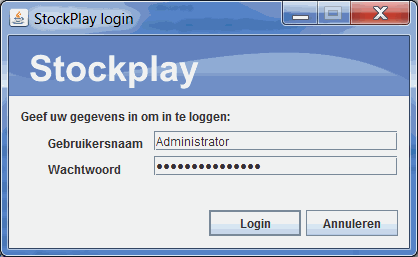
\includegraphics[width=\textwidth]{images/handleiding/handleiding1.gif}
	\caption{Abstract Syntax Tree van een voorbeeldfilter.}
\end{figure}

Het standaard openingsscherm is een overzicht van de status van de verschillende componenten, met enkele belangrijke statistieken erbij:
Opmerking: de logica in de 'backend' die achter de Start/Stop/Restart-knoppen zit is nog niet uitgewerkt.

\begin{figure}[h!]
	\centering
		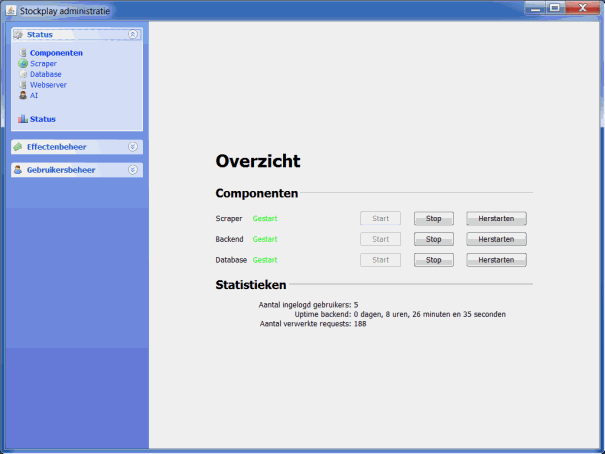
\includegraphics[width=\textwidth]{images/handleiding/handleiding7.gif}
	\caption{Abstract Syntax Tree van een voorbeeldfilter.}
\end{figure}

\section{Beheer van effecten}

Als je op "Effectenbeheer" in de linkerkolom klikt verschijnt onderstaand scherm (het inladen van de effecten duurt een grote seconde, dus even geduld). 
In het uitschuifmenu bevinden zich enkele filters waarmee je de effecten kan filteren.

\begin{figure}[h!]
	\centering
		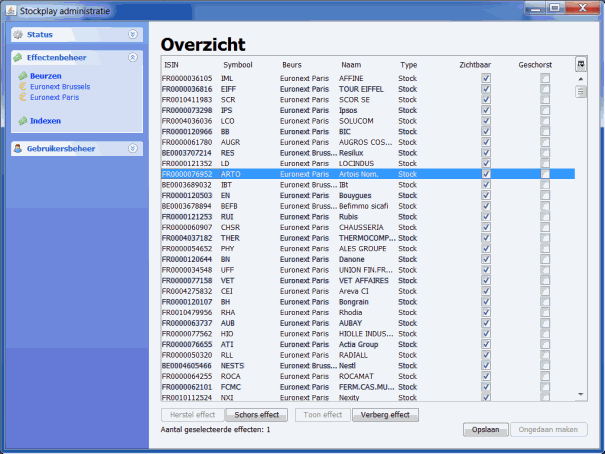
\includegraphics[width=\textwidth]{images/handleiding/handleiding6.gif}
	\caption{Abstract Syntax Tree van een voorbeeldfilter.}
\end{figure}

Op elk effect kan je de volgende acties uitvoeren:

\begin{itemize}
\item{Naam wijzigen (in de tabel klikken)}
\item{Type wijzigen (in de tabel klikken)}
\item{Zichtbaarheid wijzigen (in de tabel klikken, of de aandelen selecteren en werken met de knoppen onderaan)}
\item{Geschorst-zijn wijzigen (in de tabel klikken, of de aandelen selecteren en werken met de knoppen onderaan)}
\end{itemize}

Om de wijzigingen permanent te maken klik je vervolgens op de knop "Opslaan".

\section{Beheer van gebruikers}

Als je op "Gebruikersbeheer" in de linkerkolom klikt verschijnt onderstaand scherm.
Links klapt er nu ook weer een scala aan filters uit waarop je de gebruikers kan filteren.

\begin{figure}[h!]
	\centering
		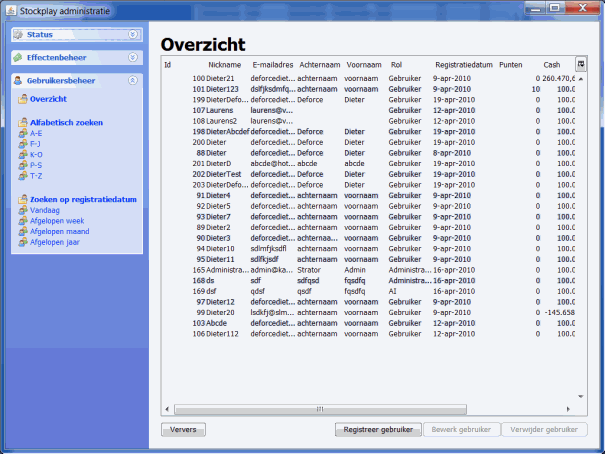
\includegraphics[width=\textwidth]{images/handleiding/handleiding5.gif}
	\caption{Abstract Syntax Tree van een voorbeeldfilter.}
\end{figure}

Opmerking: In tegenstelling tot bij effectenbeheer zijn alle acties hier direct definitief!!

De mogelijk acties zijn:
\begin{itemize}
\item{Aanmaken van een nieuwe gebruiker met 'Registreer gebruiker'. Dan verschijnt onderstaand scherm}
\end{itemize}

\begin{figure}[h!]
	\centering
		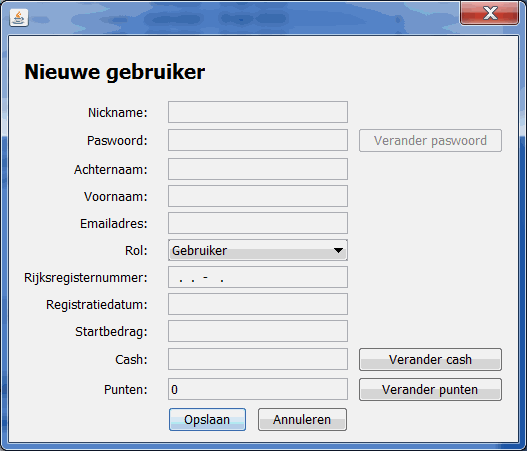
\includegraphics[width=\textwidth]{images/handleiding/handleiding4.gif}
	\caption{Abstract Syntax Tree van een voorbeeldfilter.}
\end{figure}

Om de nieuwe gebruiker te registeren moet je de velden Nickname, Paswoord, Achternaam, Voornaam en Emailadres invullen. 
De velden startbedrag, cash en punten worden bij het registeren van de gebruiker in de backend ingevuld.

Het bewerken van een gebruiker, dan verschijnt een gelijkaardig veld aan dat van "Registreer gebruiker", maar met enkele verschillen:

\begin{itemize}
\item{Om het wachtwoord te veranderen, klik je op de knop "Verander paswoord", pas daarna wordt het paswoord-veld beschikbaar}
\item{De hoeveelheid cash en punten kan worden veranderd. Onze applicatie vereist echter wel dat dit gelogged wordt, en daarom verschijnt er een nieuw scherm waar je de reden moet opgeven..}
\end{itemize}

\begin{figure}[h!]
	\centering
		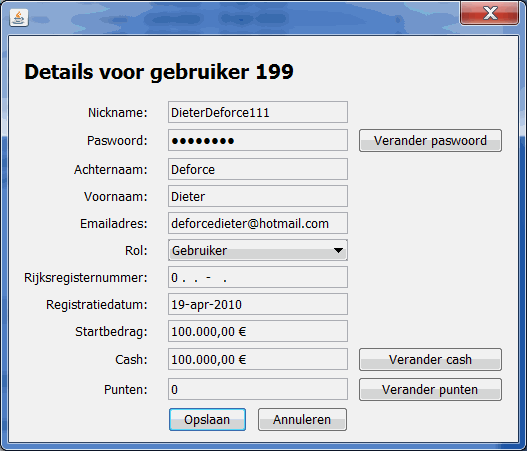
\includegraphics[width=\textwidth]{images/handleiding/handleiding3.gif}
	\caption{Abstract Syntax Tree van een voorbeeldfilter.}
\end{figure}

\begin{figure}[h!]
	\centering
		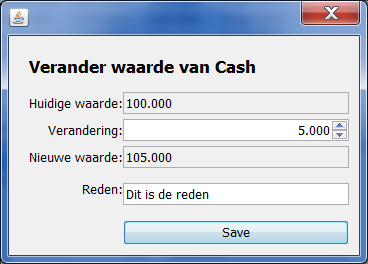
\includegraphics[width=\textwidth]{images/handleiding/handleiding2.gif}
	\caption{Abstract Syntax Tree van een voorbeeldfilter.}
\end{figure}

\chapter{Handleiding webapplicatie}

De website is bereikbaar op 'http://nernst/' 

Het eerste wat je moet doen is het je registeren. Dit kan door de "Register"-knop te gebruiken in de linkerzijbalk. Geef je gegevens in en druk op "Registreer". Log vervolgens in met je vers aangemaakte gegevens.

\section{Overzicht van effecten - opvragen van details}

Klik links op "Securities Overview" of een van de beurzen die aanwezig is in het spel om een lijst te krijgen van effecten.

Als je op de naam van een effect klikt krijg je een detailinformatie over het aandeel met het pie�e de resistance van Laurens: zijn grafiek.

De grafiek kent vele opties en laadt dynamisch zijn data in.
De grafiek kan:

\begin{itemize}
\item{uitzoomen, maximaal tot wanneer er geen data meer is voor}
\end{itemize}

\section{Aankopen van effecten}

Klik links op "Securities Overview" of een van de beurzen die aanwezig is in het spel om een lijst te krijgen van effecten. Klik op de "Buy" knop van het gewenste aandeel.

\chapter{Handleiding grafieken module op de website}

Standaard wordt een weergave gegeven van het beursverloop van de laatste 